\documentclass{ceurart}

\input{reviewing}

\sloppy

\usepackage{listings}
%% auto break lines
\lstset{breaklines=true}

% typesetting turtle code
\usepackage{color}
\usepackage[listings,skins,breakable,xparse]{tcolorbox}
\usepackage{footmisc}
\definecolor{MyLightGray}{rgb}{0.95, 0.95, 0.96}

\lstdefinelanguage{turtle}
{
    columns=fullflexible,
    keywordstyle=\color{red},
    morekeywords={@prefix,@base,@forSome,@forAll,@keywords},
    morecomment=[l]{\#},
    tabsize=4,
    alsoletter={-?}, % allowed in names
    morecomment=[s][\color{blue}]{<}{>},
    basicstyle=\ttfamily\color{black},
    %numberstyle=\color{black},
    morestring=[b][\color{black}]\",
    backgroundcolor=\color{MyLightGray},
}

\usepackage{amsmath}
\usepackage{amssymb}
\usepackage{multirow}
\usepackage{tabularx}
\usepackage{cleveref}
\usepackage{wrapfig}
\usepackage{hyperref}
\usepackage[inline]{enumitem}
\setlist{nolistsep}
\newlist{inlinelist}{enumerate*}{1}
\setlist[inlinelist,1]{label=\textit{\roman*)}}
\newlist{inlineabc}{enumerate*}{1}
\setlist[inlineabc,1]{label=\textit{\alph*)}}

\newtheorem{definition}{Definition}
\newtheorem{policy}{Policy}
\newtheorem{sotw}{SotW}

\begin{document}

\copyrightyear{2026}
\copyrightclause{Copyright for this paper by its authors.
  Use permitted under Creative Commons License Attribution 4.0
  International (CC BY 4.0).}


\conference{Fourth International Workshop on Semantics in Dataspaces (SDS 2026)}

\title{Bridging DPV and ODRL for Legally-Oriented Usage Control in Data Spaces}

\author[1]{Beatriz Esteves}[%
orcid=0000-0003-0259-7560,
email=beatriz.esteves@ugent.be,
url=https://w3id.org/people/besteves,
]
\cormark[1]
\cortext[1]{Corresponding author.}

\author[2]{Harshvardhan J. Pandit}[%
% orcid=0000-0003-0259-7560,
% email=beatriz.esteves@ugent.be,
% url=https://w3id.org/people/besteves,
]

\address[1]{IDLab, Department of Electronics and Information Systems, Ghent University -- imec, Ghent, Belgium}
\address[2]{AI Accountability Lab (AIAL), Trinity College Dublin, Dublin, Ireland}

\begin{abstract}
% Context:      Why the need is so pressing or important
Data spaces increasingly require robust usage control mechanisms to ensure that data sharing complies with legal, contractual, and governance requirements while remaining interoperable across heterogeneous systems. The W3C's ODRL Information Model 2.2 provides a domain-agnostic framework for expressing permissions, prohibitions, and obligations over assets, whereas the Data Privacy Vocabulary (DPV) offers a rich, controlled vocabulary for representing privacy and data protection concepts.
% Need:         Why something needed to be done at all
However, the lack of systematic alignment between legal-semantic vocabularies and enforceable policy languages hinders the creation of machine-readable, legally-oriented usage policies in data spaces.
% Task:         What was undertaken to address the need
This paper addresses this gap by presenting a structured mapping between DPV and ODRL that aligns DPV concepts with ODRL constructs using RDF and SKOS properties, and provides it in a machine-readable form to support implementation.
% Object:       What the present document does or covers
The mapping covers core correspondences such as DPV entities, processing, data, personal data, legal bases, purposes, technical and organisational measures, and risks, with ODRL parties, actions, assets, and left operands. 
% Findings:     What the work done yielded or revealed
By doing so, it enables the expression of legally grounded policies where DPV supplies semantically precise data protection terms, and ODRL provides the deontic and operational policy structure.
In addition, we contribute a comprehensive guidance document that specifies how DPV terms should be used within ODRL policies, including examples for constraints modelling and operator usage in accordance with ODRL profile best practices. 
% Conclusion:   What the findings mean for the audience
Together, the mapping and guidance establish a reusable foundation for implementing legally-oriented, interoperable usage control policies in data spaces. They support the creation of policy artefacts that are simultaneously machine-processable, semantically rich, and aligned with data protection and governance requirements, thereby advancing trustworthy and compliant data sharing ecosystems.
% Perspectives: What the future holds, beyond this work
% TODO: add sentences on future work on implementing mapping in policy engine
\end{abstract}

\begin{keywords}
  ODRL \sep
  DPV \sep
  usage control \sep
  regulatory compliance
\end{keywords}

\maketitle

\section{Introduction}
\label{sec:intro}

At the centre of European Commission's policy agenda,
Data spaces are emerging as a societal, legal and technical architectural paradigm,
for enabling trusted data sharing across organisational
and sectoral boundaries~\cite{farrell_european_2023}.
Their objective is to allow participants
to exchange and reuse data while maintaining control over
how that data is accessed and processed.
Achieving this balance between
data sharing and data sovereignty
requires usage control mechanisms
that can express and enforce the conditions
under which data may be used~\cite{eitel_usage_2021}.
These conditions can be derived not only from technical
but also from regulatory and contractual requirements.
In this context,
the Data Spaces Support Centre (DSSC) blueprint~\cite{data_spaces_support_centre_summary_2026}
highlights the importance of integrating legal and technical capabilities,
specifically addressing \emph{regulatory compliance and contractual frameworks}
alongside \emph{access and usage policies enforcement}.
These building blocks together aim to ensure that
the rights and obligations governing data sharing can be
defined, negotiated, and enforced in an interoperable manner.
Agreements between data providers and data consumers
must therefore be represented in a way that
supports automated interpretation, negotiation,
and enforcement during the lifecycle of data transactions.

A central challenge in this context
is the representation of such agreements
while preserving their legal meaning.
Data sharing policies must capture
permissions, prohibitions, and obligations
governing data access and usage,
while also reflecting constraints
derived from sectoral rules, 
contract law and intellectual property rights,
or data-related legislation.
At the same time,
these policies must be semantically interoperable
to support the federated nature of data spaces,
ensuring ``that data can be accurately and
consistently interpreted and used by
different people and systems''~\cite{steinbuss_semantic_2025}.
Two complementary semantic specifications provide
a promising foundation for addressing this challenge.
The W3C Open Digital Rights Language (ODRL) standard~\cite{iannella_odrl_2018}
provides a general-purpose policy model
for expressing rules
governing the use of digital assets,
including permissions, prohibitions, and obligations
which can be further restricted with contextual constraints.
Furthermore,
ODRL is recommended in the DSSC blueprint
as a standard representation for machine-readable
access and usage policies within data spaces.
While ODRL provides the structural framework for policy representation,
it intentionally remains domain- and jurisdiction-agnostic and
does not include explicit concepts related to legal compliance.
The Data Privacy Vocabulary (DPV)~\cite{pandit_data_2024}
complements ODRL by providing a rich semantic vocabulary
containing taxonomies to describe legal requirements
related to data and AI regulation.
Combining these two standards
makes it possible to bridge the gap between
legally grounded governance requirements and
machine-readable policy enforcement mechanisms.
By mapping DPV concepts to ODRL constructs,
policies can express legally meaningful constraints
while remaining compatible with existing policy evaluation and enforcement engines.
This approach aligns closely with
the DSSC blueprint's vision of interoperable data spaces
where legal agreements and
technical enforcement mechanisms
are coherently connected.

In this paper,
we argue that ODRL and DPV together
provide a suitable semantic foundation
for legally-aligned policy expression in data spaces.
We propose treating ODRL as the core policy framework
for representing permissions, prohibitions, and
obligations governing data usage,
while using DPV as the semantic layer
for modelling legal and governance concepts
referenced within those policies.
To support this integration,
we present a structured mapping between DPV and ODRL
that aligns DPV concepts with ODRL constructs,
using RDF and SKOS properties,
and provides the mapping in a machine-readable form
to facilitate implementation,
in accordance with ODRL profiling best practices~\cite{steidl_odrl_2023}.
The mapping covers core correspondences such as
DPV entities, processing operations,
data and personal data categories,
legal bases, purposes, and
the corresponding ODRL constructs
such as parties, actions, assets, and left operands.
In addition,
we provide a guidance document for the use of
DPV terms within ODRL policies,
including examples of policies that use the developed mapping.
Together,
these contributions enable data space participants
to express governance rules that are both legally meaningful
and technically enforceable,
thereby supporting scalable and
interoperable policy management
across data space infrastructures.

The remainder of this article is structured as follows:
Section~\ref{sec:background} provides an overview of applicable regulatory requirements and existing work for data protection-aligned policy modelling.
Section~\ref{sec:mapping} describes the developed mapping and its implementation as an ODRL profile.
% In Section~\ref{sec:policies}, we define a specification for ...
In Section~\ref{sec:guidelines}, we provide examples of the application of the profile and discuss the implementation of templates to validate profile-based constraints.
Finally, Section~\ref{sec:conclusions} concludes the paper and provides pointers to future research.
\section{Background \& Related Work}
\label{sec:background}

In this section, ...

\paragraph{Regulatory Compliance in Data Spaces}

Data-related legislation: GDPR~\cite{gdpr}, DGA~\cite{dga}, Data Act~\cite{data_act}

Sectorial legislation: EHDS~\cite{ehds}

\paragraph{Access and Usage Policies Enforcement}

Overview of ODRL~\cite{iannella_odrl_2018}

Overview of DPV~\cite{pandit_data_2024}

previous ODRL profiles that contributed to this mapping~\cite{esteves_odrl_2021,pandit_enhancing_2024,golpayegani_aiup_2024}

other works that use ODRL and DPV together~\cite{esteves_semantic_2025,esteves_fostering_2022,plazaortiz_authentication_2025,papagiannakopoulou_semantic_2025,yumusak_data_2024}, also there's~\cite{de_vos_odrl_2019}
\section{Mapping from DPV to ODRL}
\label{sec:mapping}

The DPV-ODRL mapping described in this paper
is being developed as part of the W3C DPVCG's activities\footnote{
    \href{https://www.w3.org/groups/cg/dpvcg/}{DPVCG's} mission is to develop vocabularies
    that support the implementation of regulations,
    standards, and approaches relevant to privacy and data protection,
    and how these are addressed in technologies, including AI.},
with the support of the W3C ODRL CG\footnote{
    \url{https://www.w3.org/groups/cg/odrl/}},
and it is available at \url{https://dev.dpvcg.org/mappings/odrl},
with \texttt{dpv-odrl} as the suggested prefix.
Furthermore,
this mapping is represented in an RDF format,
as an ODRL profile,
following the best practices documented in the
ODRL V2.2 Profile Best Practices report~\cite{steidl_odrl_2023}. 
This ensures compatibility with existing ODRL implementations
and policy evaluation mechanisms.

\subsection{Methodology}
\label{sec:methodology}

The mapping between DPV and ODRL is implemented
using semantic alignment mechanisms,
primarily through relations from the SKOS vocabulary\footnote{
    \url{http://www.w3.org/2004/02/skos/core\#}},
RDF and RDFS\footnote{
    \url{http://www.w3.org/1999/02/22-rdf-syntax-ns\#} and
    \url{http://www.w3.org/2000/01/rdf-schema\#}}, and
OWL\footnote{
    \url{http://www.w3.org/2002/07/owl\#}}.
The following alignment strategies were considered:
\begin{itemize}
    \item \textbf{Instantiation}: A \texttt{dpv-odrl} class is instantiated as an ODRL class
    \item \textbf{Specialisation}: One concept is more specific than the other
    \item \textbf{Hierarchy}: A strict ontology subclass relationship
    \item \textbf{Equivalence}: Concepts represent the same meaning
    \item \textbf{Approximation}: Concepts are very similar but not strictly equivalent
    \item \textbf{Association}: Concepts are related but not hierarchically
    \item \textbf{Disjointness}: Mutually exclusive concepts
\end{itemize}
Table~\ref{tab:mapping} provides an overview of these strategies,
the semantic property used for the mapping,
and examples.

\begin{table}[ht]
    \centering
    \caption{Mapping types of DPV and ODRL Concepts}
    \label{tab:mapping}
    \begin{tabular}{lll}
        \toprule
        \textbf{Alignment} & \textbf{Mapping Relation} & \textbf{Example} \\
        \midrule
        Instantiation & \texttt{rdf:type} & \texttt{dpv-odrl:Entity rdf:type odrl:Party .} \\
        Specialisation & \texttt{skos:broader} & \texttt{dpv-odrl:Recipient skos:broader odrl:recipient .} \\
        Hierarchy & \texttt{rdfs:subClassOf} & \texttt{dpv-odrl:NDA rdfs:subClassOf odrl:Policy .} \\
        Equivalence & \texttt{skos:exactMatch} & \texttt{dpv-odrl:Agent skos:exactMatch dpv:Agent .} \\
        Approximation & \texttt{skos:closeMatch} & \texttt{dpv-odrl:Use skos:closeMatch odrl:use .} \\
        Association & \texttt{skos:related} & \texttt{dpv-odrl:Duration skos:related odrl:elapsedTime .} \\
        Disjointness & \texttt{owl:disjointWith} & \texttt{dpv-odrl:NDA owl:disjointWith (odrl:Offer, ...) .} \\
        \bottomrule
    \end{tabular}
\end{table}
% Disjointment: \texttt{$P_1 \cap P_i = \varnothing \quad \forall i \neq 1$}

\subsection{DPV-ODRL Profile}
\label{sec:profile}

Through the mapping described in the previous section,
DPV concepts can function within ODRL policies as:
\begin{inlinelist}
    \item parties,
    \item actions,
    \item assets,
    \item left operands,
    \item rules, and
    \item policy types
\end{inlinelist}.
Figure~\ref{fig:mapping}
provides an overview of this mapping where all DPV taxonomies
are mapped into one or more of the previously mentioned ODRL constructs.

\begin{figure}[ht]
    \centering
    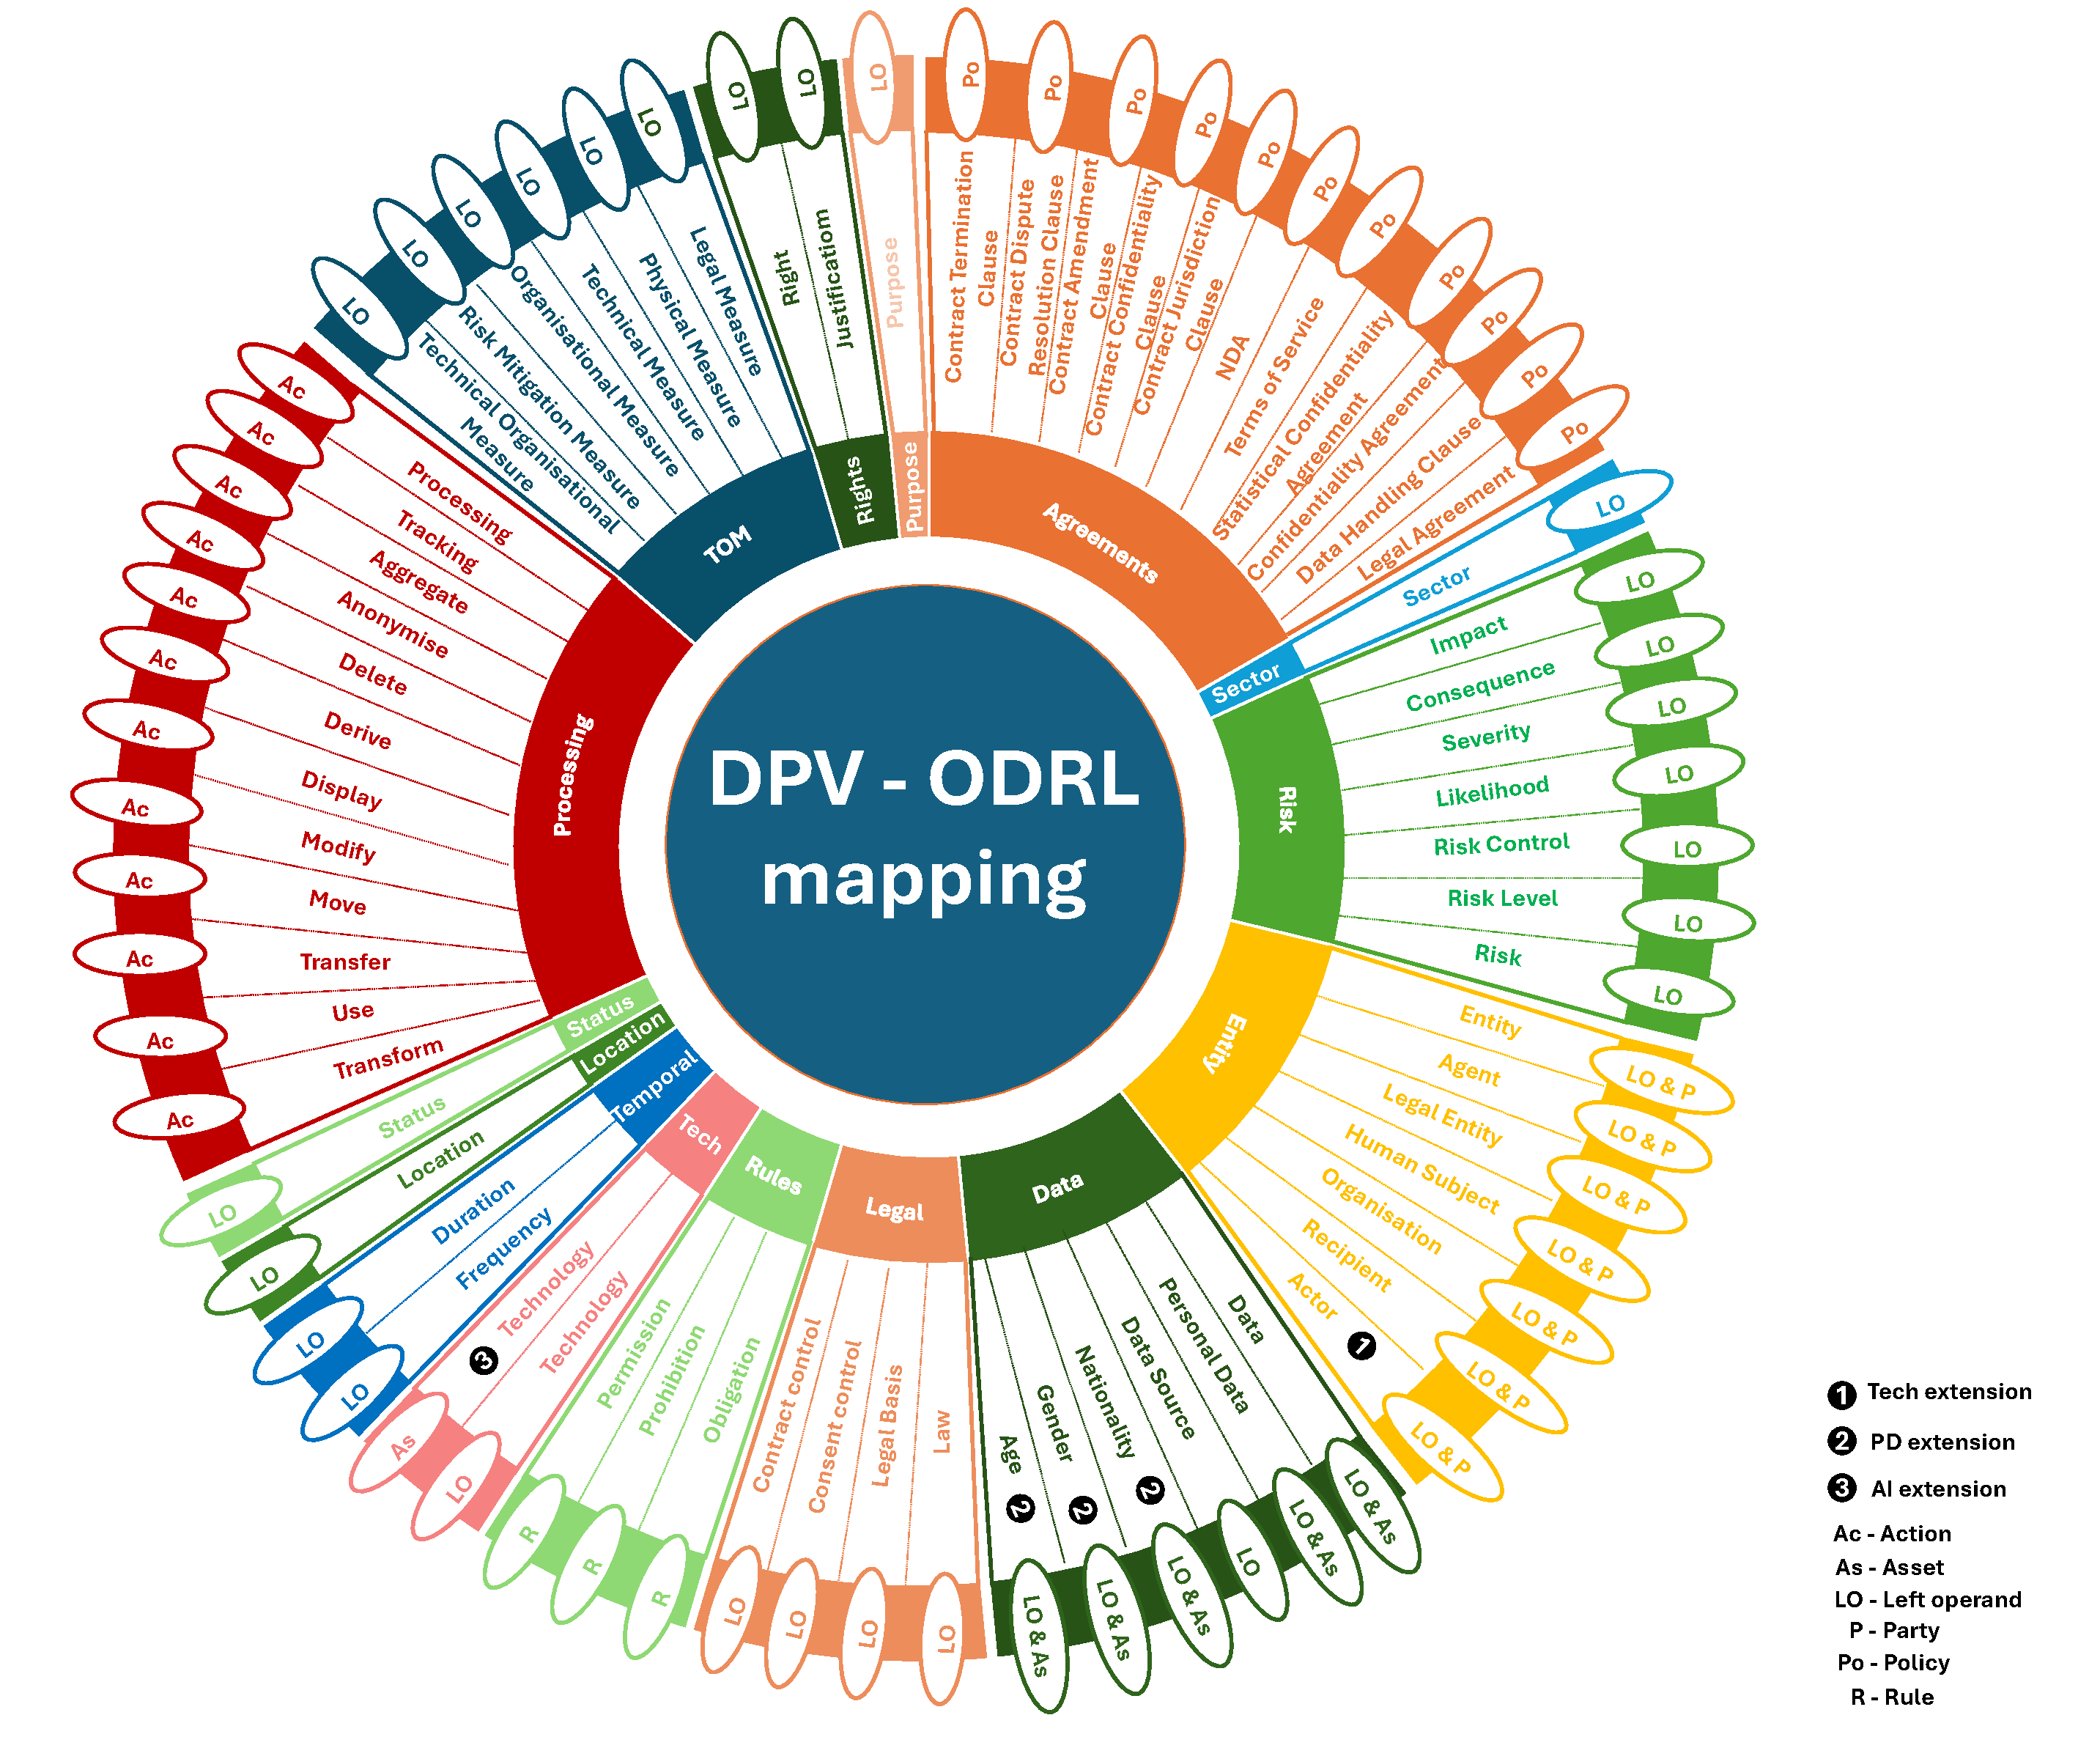
\includegraphics[width=\linewidth]{overview_cropped.pdf}
    \caption{Overview of DPV-ODRL mapping: the inner layer groups the terms by taxonomy, the middle layer contains the mapped DPV terms, and the outer layer contains the mapping to ODRL constructs.}
    \label{fig:mapping}
\end{figure}

\paragraph{Entities and Legal Roles}

DPV defines entities and legal roles
representing stakeholders involved in data processing activities,
such as individuals, organisations, institutions, or authorities.
As such,
they can be mapped as \texttt{odrl:Party} instances
and used as \texttt{odrl:assigner} or \texttt{odrl:assignee} of ODRL policies.
Furthermore,
due to the hierarchical structure of DPV,
certain entity concepts can be used as
left operands to filter ODRL party collections.
For example,
when a party collection contains multiple human subjects of different types,
the use of \texttt{dpv-odrl:HumanSubject} as the left operand
and \texttt{dpv:Patient} as the right operand
enables the specification of an ODRL policy
that applies exclusively to subjects of this particular type.
Listing~\ref{lst:entity} provides an example of a
DPV-ODRL mapping for entity concepts.
In this case,
\texttt{dpv-odrl:Recipient},
the equivalent to \texttt{dpv:Recipient},
is instantiated
as a \texttt{odrl:Party} and as a \texttt{odrl:LeftOperand},
and has a narrower scope than \texttt{odrl:recipient},
i.e., the right operand of \texttt{odrl:recipient}
is not restricted to a particular vocabulary,
while \texttt{dpv-odrl:Recipient} should require
a \texttt{dpv:Entity} as the right operand.

\begin{scriptsize}
\begin{lstlisting}[language=turtle, caption=DPV-ODRL mapping for the Recipient concept., label=lst:entity]
dpv-odrl:Recipient a odrl:Party, odrl:LeftOperand, skos:Concept ;
	skos:exactMatch dpv:Recipient ;
	skos:broader odrl:recipient .
    # add scope, e.g., which operators and right operand should be used
\end{lstlisting}
\end{scriptsize}

\paragraph{Processing Operations}

DPV processing concepts describe
operations that may be performed on data,
such as aggregation, deletion, transformation, or transfer.
These operations naturally correspond to ODRL actions and
can therefore be used to define
permitted, prohibited or mandatory activities within policies.
Furthermore, 
a few DPV processing terms closely correspond to existing ODRL actions,
allowing them to be related using the \texttt{skos:closeMatch}~---~%
Table~\ref{tab:processing} contains an overview of these terms.
Listing~\ref{lst:action} provides an example of a
DPV-ODRL mapping for a processing operation.
In this case,
\texttt{dpv-odrl:Use},
the equivalent to \texttt{dpv:Use},
is instantiated as an \texttt{odrl:Action} and
has a similar ODRL concept, i.e., \texttt{odrl:use}.

\begin{scriptsize}
\begin{lstlisting}[language=turtle, caption=DPV-ODRL mapping for the Use concept., label=lst:action]
dpv-odrl:Use a odrl:Action, skos:Concept ;
	skos:exactMatch dpv:Use ;
	skos:closeMatch odrl:use .
\end{lstlisting}
\end{scriptsize}

\begin{table}[ht]
    \centering
    \caption{Mapping of DPV processing operations to ODRL actions.}
    \label{tab:processing}
    \begin{tabular}{lll}
        \toprule
        \textbf{ODRL Concept} & \textbf{DPV Concept} & \textbf{Mapping Type} \\
        \midrule
        odrl:acceptTracking & dpv:Tracking & skos:closeMatch \\
        odrl:aggregate & dpv:Aggregate & skos:closeMatch \\
        odrl:anonymize & dpv:Anonymise & skos:closeMatch \\
        odrl:delete & dpv:Delete & skos:closeMatch \\
        odrl:derive & dpv:Derive & skos:closeMatch \\
        odrl:display & dpv:Display & skos:closeMatch \\
        odrl:modify & dpv:Modify & skos:closeMatch \\
        odrl:move & dpv:Move & skos:closeMatch \\
        odrl:transfer & dpv:Transfer & skos:closeMatch \\
        odrl:transform & dpv:Transform & skos:closeMatch \\
        odrl:use & dpv:Use & skos:closeMatch \\
        \bottomrule
    \end{tabular}
\end{table}

\paragraph{Data and Technologies}

In ODRL,
assets represent the resources targeted by policies.
On the other hand,
DPV provides a comprehensive taxonomy for describing data,
including categories of personal and non-personal data,
as well as a Personal Data Categories extension\footnote{
    \url{https://w3id.org/dpv/pd}},
which provides additional concepts to represent different types of personal data,
e.g., social, demographic, financial, or health-related data categories.
These concepts can therefore be mapped to ODRL assets,
but can also be used as left operands to refine asset or party collections
to specific demographic groups, e.g.,
to restrict the usage of a certain asset to parties which are over 18.
% TODO: include example in the next section that can be referenced here
Furthermore,
DPV provides technology-related concepts
that can be used to denote the use of any technological resources,
including AI systems.
These concepts can also be used as assets within ODRL policies
to specify conditions governing the use of such resources.
Furthermore, DPV's Technology\footnote{
    \url{https://w3id.org/dpv/tech}}
and AI Technology\footnote{
    \url{https://w3id.org/dpv/ai}}
extensions introduce additional technological concepts
that can be employed as assets or as further constraints in ODRL policies.
For example,
a policy may specify that a given asset may only be used for training an AI model.

\paragraph{Contextual and Governance-related Constraints}

The majority of DPV taxonomies yet to be discussed in this section
are mapped as ODRL left operands to further constrain ODRL policies.
The following list provides an overview of these taxonomies and
their utility to restrict ODRL policies:
\begin{itemize}
    \item \textbf{Purpose:} Purpose limitation is a central principle in many data protection frameworks, particularly the GDPR. DPV includes an extensive taxonomy of purposes, which can be integrated into ODRL policies to constrain data or technology usage to a particular purpose or set of purposes. This alignment enables the expression of policies such as allowing the use of a dataset exclusively for research or restricting its use to statistical analysis.
    \item \textbf{Technical and Organisational Measures:} Data protection regulations frequently require the implementation of safeguards such as encryption, authentication mechanisms, or organisational controls. DPV models such safeguards as technical and organisational measures (TOMs), which can be used as constraints within ODRL policies for, e.g., permitting access to a dataset only when multi-factor authentication is implemented.
    \item \textbf{Legal and Jurisdictional Constraints:} DPV location concepts can restrict asset usage to specific locations or jurisdictions, supported by the Location\footnote{\url{https://w3id.org/dpv/loc}} extension that contains concepts to represent countries and regions based on ISO 3166. Additionally, DPV provides concepts for representing applicable laws and legal bases for processing activities, with the Legal\footnote{\url{https://w3id.org/dpv/legal}} extensions supporting the modelling of laws and authorities across jurisdictions.
    \item \textbf{Time-based Context:} Temporal aspects of policies, including duration and frequency of usage, can also be represented through DPV concepts. These mappings allow policies to define how long data may be used or how often certain operations may occur. Furthermore, these DPV concepts can be related to a few ODRL left operands in a non-hierarchical way, e.g., \texttt{dpv:Duration} is related to \texttt{odrl:elapsedTime}. Listing~\ref{lst:duration} provides the DPV-ODRL mapping for duration, where \texttt{dpv-odrl:Duration}, the equivalent to \texttt{dpv:Duration}, is instantiated as an \texttt{odrl:LeftOperand} and has related ODRL concepts, i.e., \texttt{odrl:elapsedTime} and \texttt{odrl:count}.
    \item \textbf{Rights and Risks:} DPV includes concepts representing risks, rights, and justifications associated with processing activities. They can be used to justify the exercising of a certain right, e.g., a data subject wants to exercise their right to erasure given that the processing of their personal data is no longer required, or to restrict the use of assets when risk levels exceed certain thresholds.
    \item \textbf{Sector and Status:} DPV sector concepts can be used to permit or restrict asset usage based on the application domain. The AI Act\footnote{\url{https://w3id.org/dpv/legal/eu/aiact}} extension provides sector-related concepts, such as education and employment, to represent these domains. Additionally, DPV status concepts can indicate the state of processes or activities, enabling policies to constrain asset usage based on conditions such as the status of given consent.
\end{itemize}
A detailed list of these mappings
is available at \url{https://dev.dpvcg.org/mappings/odrl}
and can be observed in Figure~\ref{fig:mapping}.

\begin{scriptsize}
\begin{lstlisting}[language=turtle, caption=DPV-ODRL mapping for the Duration concept.,  label=lst:duration]
dpv-odrl:Duration a odrl:LeftOperand, skos:Concept ;
    skos:exactMatch dpv:Duration ;
	skos:related odrl:elapsedTime, odrl:count .
\end{lstlisting}
\end{scriptsize}

\paragraph{Rules}

\begin{scriptsize}
\begin{lstlisting}[language=turtle, caption=Secondary use policy for purposes associated with healthcare scientific research.,  label=lst:rule]
dpv-odrl:Obligation skos:exactMatch dpv:Obligation ;
	skos:closeMatch odrl:Duty .
\end{lstlisting}
\end{scriptsize}

\paragraph{Agreements}

\begin{scriptsize}
\begin{lstlisting}[language=turtle, caption=Secondary use policy for purposes associated with healthcare scientific research.,  label=lst:policy]
dpv-odrl:NDA a rdfs:Class, skos:Concept ;
    skos:exactMatch dpv:NDA ;
	rdfs:subClassOf odrl:Policy ;
	owl:disjointWith odrl:Agreement, odrl:Offer, odrl:Privacy, odrl:Request, odrl:Ticket, odrl:Assertion,
	dpv-odrl:ContractConfidentialityClause, dpv-odrl:ContractDisputeResolutionClause,
	dpv-odrl:ContractJurisdictionClause, dpv-odrl:ContractTerminationClause,
	dpv-odrl:TermsOfService, dpv-odrl:DataHandlingClause, dpv-odrl:LegalAgreement,
	dpv-odrl:ConfidentialityAgreement, dpv-odrl:NDA, dpv-odrl:StatisticalConfidentialityAgreement .
\end{lstlisting}
\end{scriptsize}
% \section{Legal Agreements as Actionable Policies}
\label{sec:policies}

This section outlines ...


\section{Usage Guidelines}
\label{sec:guidelines}

In addition to the DPV-ODRL mapping
described in the previous section,
we provide a guidance document 
at \url{https://dev.dpvcg.org/guides/dpv-odrl}
with examples of ODRL policies that use the developed mapping
and conform with the ODRL standard.
In this section,
we reproduce a few of these examples to 
showcase the usefulness of this work
to tackle legal compliance enforcement
in data spaces.

Listing~\ref{lst:partycollection}
provides an example of a DPV-ODRL policy,
where a data holder allows the usage of a certain asset,
i.e., \texttt{ex:research-dataset},
only for the purpose of
\texttt{dpv:ResearchAndDevelopment}
and only for data users which are classified as 
\texttt{dpv:AcademicScientificOrganisation}.

\begin{scriptsize}
\begin{lstlisting}[language=turtle, caption=Purpose-restricted agreement with a party collection refinement., label=lst:partycollection]
ex:policy-partycollection a odrl:Agreement ;
    odrl:uid ex:policy-partycollection ;
    odrl:profile dpv-odrl: ;
    odrl:permission [
        odrl:assigner ex:data-holder ;
        odrl:assignee [ 
            a odrl:PartyCollection ;
            odrl:source ex:entities ;
            odrl:refinement [
                odrl:leftOperand dpv-odrl:Entity ;
                odrl:operator odrl:isA ;
                odrl:rightOperand dpv:AcademicScientificOrganisation ] ] ;
        odrl:target ex:research-dataset ;
        odrl:action dpv-odrl:Use ;
        odrl:constraint [
            odrl:leftOperand dpv-odrl:Purpose ;
            odrl:operator odrl:isA ;
            odrl:rightOperand dpv:ResearchAndDevelopment ] ] .
\end{lstlisting}
\end{scriptsize}

Listing~\ref{lst:assetcollection}
provides an example of a DPV-ODRL policy,
where a data subject allows the usage of elements
of a certain asset collection,
i.e., \texttt{ex:data-catalog},
that are instances of health record data,
i.e., \texttt{pd:HealthRecord}.

\begin{scriptsize}
\begin{lstlisting}[language=turtle, caption=Policy with a DPV-ODRL-based asset collection refinement on personal data type., label=lst:assetcollection]
ex:policy-assetcollection a odrl:Policy ;
    odrl:uid ex:policy-assetcollection ;
    odrl:profile dpv-odrl: ;
    odrl:permission [
        odrl:target [ 
            a odrl:AssetCollection ;
            odrl:source ex:data-catalog ;
            odrl:refinement [
                odrl:leftOperand dpv-odrl:PersonalData ;
                odrl:operator odrl:isA ;
                odrl:rightOperand pd:HealthRecord ]] ;
        odrl:assigner ex:data-subject ;
        odrl:action dpv-odrl:Use ] .
\end{lstlisting}
\end{scriptsize}

Listing~\ref{lst:righterasure} contains an
example specifying an agreement between
a data subject and
a data controller,
where the data controller has the obligation
to delete the data subject data,
given that the latter exercised their
GDPR right to erasure, i.e., \texttt{eu-gdpr:A17},
supported by a non-necessity justification,
i.e., \texttt{eu-gdpr:JustificationA17NonNecessity},
which can be used in such a request
when the involved personal data is no longer necessary
in relation to the purposes for which it was initially collected
or otherwise processed.

\begin{scriptsize}
\begin{lstlisting}[language=turtle, caption=Obligation-based policy for the exercising of a right and related justification., label=lst:righterasure]
ex:policy-right-erasure-justification a odrl:Agreement ;
    odrl:uid ex:policy-right-erasure-justification ;
    odrl:profile dpv-odrl: ;
    odrl:obligation [
        odrl:assigner ex:subject ;
        odrl:assignee ex:controller ;
        odrl:target ex:subject-data ;
        odrl:action dpv-odrl:Delete ;
        odrl:constraint [
            odrl:leftOperand dpv-odrl:Right ;
            odrl:operator odrl:eq ;
            odrl:rightOperand eu-gdpr:A17 ], [
            odrl:leftOperand dpv-odrl:Justification ;
            odrl:operator odrl:eq ;
            odrl:rightOperand eu-gdpr:JustificationA17NonNecessity ] ] .
\end{lstlisting}
\end{scriptsize}

Finally,
we provide a policy catalog at
\url{https://github.com/besteves4/SDS2026-DPV-ODRL-mapping}
that contains an example policy for each mapped concept.

\subsection{SHACL Shapes for Constraint Validation}
\label{sec:shacl}

Beyond specifying examples,
the guidance document
recommends the usage of SHACL\footnote{
    \url{https://www.w3.org/TR/shacl/}
} shapes
to validate DPV-ODRL-based policies.
While such shapes already exist
to validate core ODRL constructs\footnote{See \url{
    https://github.com/oeg-upm/licensius/blob/master/odrlapi/src/main/resources/shapes.ttl}},
the same exercise is needed for
the policies described in this work,
in particular to validate the usage of constraints,
as previously discussed in Section~\ref{sec:operators}.
In this context,
the ODRL vocabulary has a set of 12
defined constraint operators to express
the relation between left and right operands.
Given that multiple operators
can be used to restrict this relation,
the left operand and operator usage
should be refined for each left operand,
e.g., the \texttt{odrl:isA} operator
should not be used with the
\texttt{dpv-odrl:Frequency} left operand.
Listing~\ref{lst:shacl}
provides a template 
for a SPARQL-based SHACL constraint
that can be used to
detect the usage of an invalid operator
for a given left operand.

\pagebreak

\begin{scriptsize}
\begin{lstlisting}[language=turtle, caption=Template shape to detect the usage of an invalid operator for a given left operand., label=lst:shacl]
ex:ConstraintShapeTemplate a sh:NodeShape ;
    sh:targetClass odrl:Constraint ;
    sh:sparql [
        a sh:SPARQLConstraint ;
        sh:message "Invalid operator for given left operand." ;
        sh:prefixes odrl: ;
        sh:select """
            SELECT $this WHERE {
                $this odrl:leftOperand <LEFT_OPERAND> .
                $this odrl:operator ?op .
                FILTER(?op NOT IN (<ALLOWED_OPERATORS>))
            }
        """ ;
    ] .
\end{lstlisting}
\end{scriptsize}
\section{Conclusions and Future Work}
\label{sec:conclusions}

This article presents a structured integration of the Data Privacy Vocabulary with the Open Digital Rights Language to enable the representation of legally grounded, machine-readable usage control policies in data spaces. By defining a comprehensive mapping between DPV taxonomies and ODRL constructs, and formalising it as an interoperable ODRL profile, the work bridges the gap between legal semantics and enforceable policy representations. The resulting approach allows policies to capture permissions, prohibitions, and obligations enriched with domain-specific concepts such as purposes, legal bases, risks, and technical measures, thereby supporting the expression of compliance requirements derived from data protection and governance frameworks. Overall, this contribution provides a reusable and extensible foundation for aligning legal, organisational, and technical perspectives in the design of trustworthy and interoperable data sharing ecosystems.

Future work will focus on the implementation and evaluation of this profile within interoperable ODRL policy engines~\cite{slabbinck_interoperable_2025} to support automated policy interpretation, validation, and enforcement across heterogeneous data space infrastructures. This includes extending existing ODRL engines to natively support DPV-based semantics and integrating SHACL-based validation mechanisms for constraint checking. Additionally, further research is needed to assess scalability and interoperability across different data space implementations, as well as to explore integration with data negotiation protocols and trust frameworks. These efforts will contribute to operationalising the proposed profile and advancing practical, standards-based solutions for legally compliant usage control in real-world data spaces.

% \section*{Acknowledgments}
% This research was funded by SolidLab Vlaanderen (Flemish Government, EWI and RRF project VV023/10) and by the imec.icon project PACSOI (HBC.2023.0752), which was co-financed by imec and VLAIO and brings together the following partners: FAQIR Foundation, FAQIR Institute, MoveUP, Byteflies, AContrario, and Ghent University -- IDLab.

\section*{Declaration on Generative AI}
During the preparation of this work, the author(s) used Grammarly in order to: Grammar and spelling check. After using this tool/service, the author(s) reviewed and edited the content as needed and take(s) full responsibility for the publication's content.

\bibliography{references}

\end{document}
